\documentclass[a4paper,11pt]{article}
\pdfoutput=1 % if your are submitting a pdflatex (i.e.~if you have
% images in pdf, png or jpg format)

\usepackage{jheppub,amsthm} % for details on the use of the package, please
% see the JHEP-author-manual

\usepackage[utf8]{inputenc}
\usepackage{bm}
\usepackage{booktabs,multirow, quotes}

\usepackage[english]{babel}
\usepackage{amsmath,amssymb,graphicx,xcolor,alltt}
\usepackage{framed}

%%%%%%%%%% Start TeXmacs macros
%\catcode`\<=\active \def<{
%\fontencoding{T1}\selectfont\symbol{60}\fontencoding{\encodingdefault}}
\newcommand{\longminus}{{-\!\!-}}
\newcommand{\tmop}[1]{\ensuremath{\operatorname{#1}}}
\newcommand{\dd}{\mathrm{d}}
\newcommand{\ii}{\mathrm{i}}
\newcommand{\ketbra}[2]{\lvert #1\rangle\!\langle #2\rvert}


\newcommand{\beq}{\begin{equation}}
\newcommand{\eeq}{\end{equation}}
\newcommand{\bea}{\begin{eqnarray}}
\newcommand{\ea}{\end{eqnarray}}


\theoremstyle{remark}
\newtheorem{remark}{Remark}[section]
\newtheorem{example}{Example}[section]
\theoremstyle{theorem}
\newtheorem{lemma}{Lemma}[section]

%%%%%%%%%% End TeXmacs macros
\def\red{\color{red}}

\newcommand{\SR}[1]{{\red \bf [{SR:} #1]}}
\newcommand{\junchen}[1]{\textcolor{blue}{\textbf{[JR: #1]}}}
\def\cO{\mathcal{O}}

\makeatletter
\def\@fpheader{\ }
\makeatother

\title{Optimization}

 
\author{Junchen Rong$^1$,}
\author{Slava Rychkov$^2$}

% The "\note" macro will give a warning: "Ignoring empty anchor..."
% you can safely ignore it.

\affiliation{$^1$CPHT, CNRS, \'Ecole Polytechnique, Institut Polytechnique de Paris, Palaiseau, France\\
$^2$Institut des Hautes \'Etudes Scientifiques, 91440 Bures-sur-Yvette, France}


% e-mail addresses: one for each author, in the same order as the authors
\emailAdd{junchen.rong@polytechnique.edu}
\emailAdd{slava@ihes.fr}




\abstract{aaa}%This is a note on the measurement of 3pt function using Rydberg atom experiments.}



\begin{document} 
	
	\maketitle
	
	\flushbottom


\flushbottom
We save the phase diagram in Fig.~\ref{fig:phasediagram} for later use.
\begin{figure}[t]
  \centering
  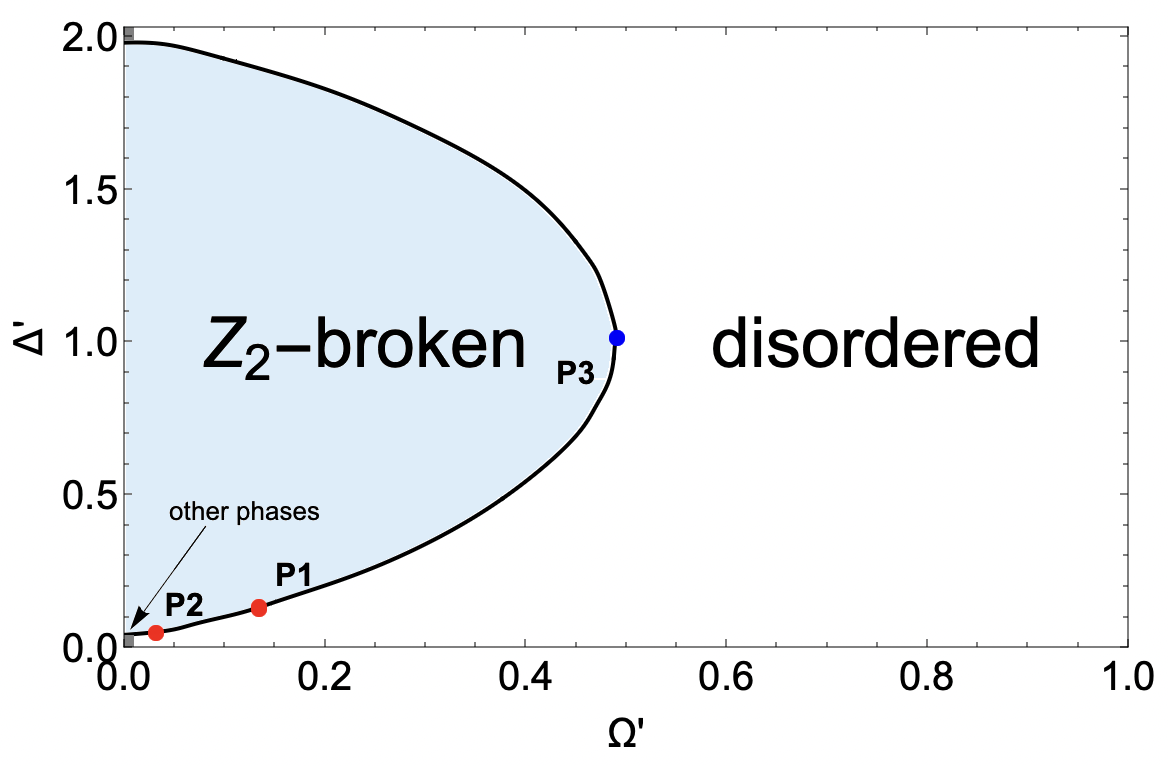
\includegraphics[width=0.6\columnwidth]{phase_diagram.png}
  \caption{The phase diagram.}
  \label{fig:phasediagram}
\end{figure}


We parametrize the two-segment curve (Path A) as:
\begin{align}
0\leq q\leq1:&\quad
\Omega(q)=0.133q,\qquad \Delta(q)=-0.403, \nonumber\\
1\leq q\leq2:&\quad
\Omega(q)=0.133,\qquad \Delta(q)=-0.403+0.54(q-1). 
\end{align}
The final point is therefore P1$=(\Omega,\Delta)=(0.133,0.137)$, which is critical.
We take the three-segment path  (Path B) to be 
\begin{align}
0\leq q\leq1:&\quad (\Omega,\Delta)=(q,-1), \nonumber\\
1\leq q\leq2:&\quad (\Omega,\Delta)=\bigl(1,-1+(\zeta(6)+1)(q-1)\bigr), \nonumber\\
2\leq q\leq3:&\quad (\Omega,\Delta)=\bigl(1-0.512(q-2),\zeta(6)\bigr). 
\end{align}
The final point  P3$=(\Omega,\Delta)=(0.488,\zeta(6))$ is also a critical point.

 
\begin{figure}[t]
  \centering
  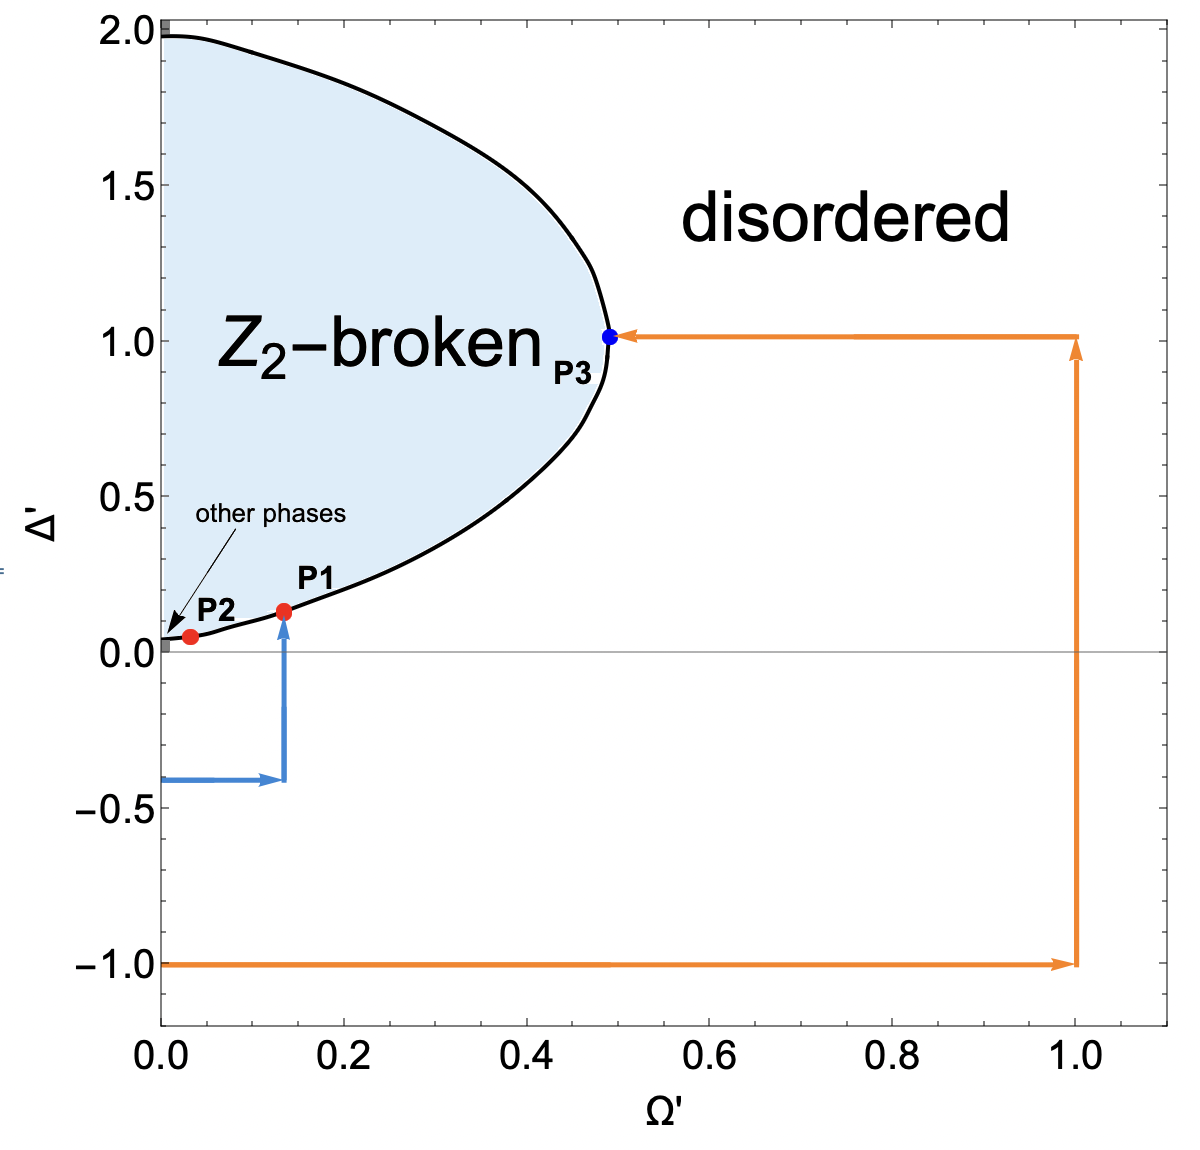
\includegraphics[width=0.6\columnwidth]{ramping_curves.png}
  \caption{Ramping paths in the $(\Omega,\Delta)$ plane. Arrows indicate the direction of evolution.}
  \label{fig:paths}
\end{figure}


\section{Matrix free time evolution of the ground state}
We use a matrix-free approach to calculate the time evolution of the ground state.  At $L=24$, the dimension of the zero-momentum, reflection-positive Hilbert space is $D=352{,}698$. The $352{,}698\times352{,}698$ Hamiltonian is never explicitly constructed and stored.
The Schrödinger equation is
\[i\hbar\frac{\partial}{\partial t}\lvert\psi(t)\rangle
=
U H(t)\lvert\psi(t)\rangle .\]
The experimental platform has $U=\hbar \cdot 75.69 MHz$ as we explained in the main text. In this appendix, we take $\hat{t} =t\cdot U/\hbar$ to be the dimensionless time. We will drop the hat for simplicity. 
Formally, we can solve the equation 
\[
\lvert\psi(t)\rangle
=
\mathcal{U}(t,0)\lvert\psi(0)\rangle ,\]
with the time evolution operator,
\[
\mathcal{U}(t,0)
=
\mathcal T
\exp\left[
-i\int_0^t H(t')\,dt'
\right].
\]Here \(\mathcal T\) is the time-ordering operator. It is necessary because, in general,
\[
[H(t_1),H(t_2)]\neq 0.
\]
Numerically, we use the fourth-order commutator-free Magnus (CF4) scheme
to take into account this time ordering. The error will be fourth-order in time steps $dt$~\cite{BlanesMoan2006,AlvermannFehske2011}.

 It samples the time-dependent Hamiltonian at two Gauss--Legendre nodes inside the interval,
\begin{equation*}
t_{n,1}=t_n+c_1dt,\qquad t_{n,2}=t_n+c_2 dt,
\end{equation*}
and we define
\begin{align*}
H_1&=H\!\left(\Omega(t_{n,1}),\Delta(t_{n,1})\right),\\
H_2&=H\!\left(\Omega(t_{n,2}),\Delta(t_{n,2})\right).
\end{align*}
Thus $H_1$ is the Hamiltonian evaluated at the earlier node and $H_2$ is the Hamiltonian at the later node. With
\begin{equation}\label{eq:cf4}
 \vert \psi_{n+1}\rangle=
 e^{-i dt (a_1 H_1+a_2 H_2)}
 e^{-i dt (a_2H_1+a_1H_2)} 
\vert \psi_n\rangle,
\end{equation}
with 
$$
c_{1,2}={}\frac12\mp\frac{\sqrt3}{6}, \quad
a_{1,2}=\frac{3\mp2\sqrt3}{12}.
$$
Equation~\eqref{eq:cf4} combines two exponentials with the two generators
\begin{equation*}
G_A=a_2H_1+a_1H_2,
\qquad
G_B=a_1H_1+a_2H_2.
\end{equation*}
The first operation on $\vert\psi_n\rangle$ is $e^{-\ii hG_A}$, followed by $e^{-\ii hG_B}$.  Their product reproduces the time-ordered propagator with local error $O(h^5)$ and hence global error $O(h^4)$, without evaluating an explicit commutator. 

The remaining problem is to apply $e^{-\ii hG}$ to the state. Forming the dense matrix exponential is expensive.
Instead, for the input vector $\vert v\rangle$, we use the order-$m$ Krylov space
\begin{equation}
\mathcal K_m(G,v)=\operatorname{span}\left\{
\vert v\rangle,G\vert v\rangle,\ldots,G^{m-1}\vert v\rangle
\right\},
\label{eq:krylovspace}
\end{equation}
which can be calculated in a matrix-free manner. 
This choice follows directly from the power series of the exponential: every term in $e^{-\ii hG}\vert v\rangle$ is proportional to one of the vectors appearing in Eq.~\eqref{eq:krylovspace}.  The approximation is therefore tailored to the action of the exponential.

For Hermitian $G$, the Lanczos iteration constructs an orthonormal basis
\begin{equation*}
V_m=(\vert v_1\rangle,\ldots,\vert v_m\rangle),
\qquad
\vert v_1\rangle=\frac{\vert v\rangle}{\lVert v\rVert},
\end{equation*}
using the three-term recurrence \cite{Lanczos1950}
\begin{equation}
G\vert v_j\rangle
=\beta_{j-1}\vert v_{j-1}\rangle
+\alpha_j\vert v_j\rangle
+\beta_j\vert v_{j+1}\rangle.
\label{eq:lanczosrecurrence}
\end{equation}
Consequently, the projected representation of $G$,
\begin{equation}
T_m=V_m^\dagger G V_m
=
\begin{pmatrix}
\alpha_1&\beta_1&&0\\
\beta_1&\alpha_2&\ddots&\\
&\ddots&\ddots&\beta_{m-1}\\
0&&\beta_{m-1}&\alpha_m
\end{pmatrix},
\label{eq:tridiagonal}
\end{equation}
is an $m\times m$ real symmetric tridiagonal matrix.  Here $V_m$ is a $D\times m$ matrix only in notation: numerically, its columns are stored as $m$ Lanczos vectors.
The exponential action is then approximated as \cite{HochbruckLubich1997}
\begin{equation}
e^{-\ii hG}\vert v\rangle
\simeq
\lVert v\rVert V_m e^{-\ii hT_m}\bm e_1,
\qquad
\bm e_1=(1,0,\ldots,0)^T.
\label{eq:krylovexp}
\end{equation}
Only the small $m\times m$ matrix $T_m$ is exponentiated.  Constructing it requires repeated products $G\vert w\rangle$, and each such product is evaluated as a weighted sum of the already available matrix-free actions $H_1\vert w\rangle$ and $H_2\vert w\rangle$.  Neither Hamiltonian, nor generator, nor exponential is stored as a full $D\times D$ matrix.  Krylov approximations to matrix-exponential actions and their convergence are analyzed in Ref.~\cite{HochbruckLubich1997}; the same combination with commutator-free propagators is discussed explicitly in Ref.~\cite{AlvermannFehske2011}.

We reduce the remaining CF4 time-step error by Richardson extrapolation \cite{Richardson1911}.  Let $F_h$ denote the final ground-state fidelity obtained for a fixed physical ramp duration $T$ using nominal CF4 step $h$.  
We successively decrease the time step to ensure that the error is in the asymptotic fourth order in $h$. The result is then approximately
\begin{align*}
F_{dt}&=F_{d t\to0}+C dt^4+\text{higher-order terms},\\
F_{dt/2}&=F_{\Delta t\to0}+\frac{C dt^4}{16}
+\text{higher-order terms}.
\end{align*}
Here $F_{d t\to0}$ is the fidelity obtained in the zero-numerical-step-size limit.  Doing the time evolution at both $dt$ and $dt/2$ allows us to estimate $ C$ and find $F_{d t\to0}$.

We can use this method to evolve the experimental curve:
\begin{align}
{\rm Segment 1}: \quad& \Omega'(t)=0.133 \frac{t}{2\tilde{t}}, \quad \Delta'(t)=\Delta_i, \nonumber\\
{\rm Segment 2}: \quad& \Omega'(t)=0.133, \quad \Delta'(t)=\frac{G_i \Delta_f (t-2\tilde{t}) + G_f \Delta_i (7\tilde{t} - t)}{ G_i (t-2\tilde{t}) + G_f (7 \tilde{t}-t)},
\end{align}
with 
\begin{equation}
\Delta_i = -0.403,~\Delta_f = 0.137,~G_i =0.45389,~G_f = 0.03039, \quad {\rm and}~ \tilde{t}=75.69.
\end{equation}
Here $G_i$ and $G_f$ are the energy gaps, and $\tilde{t}=75.69$ corresponds to $1 \mu s$ in physical units. Using $dt=1$, we get 
\[
|c_0|=0.9952060572,\qquad
|c_1|=0.0653074360,\qquad
|c_2|=0.0361195216.
\]
Let us define the lattice operator 
$$
 s_i = (-1)^i (Z_i -\langle Z_i \rangle).
$$
We can calculate the error on its two-point function introduced by ramping, which is 
\begin{equation}\label{def:error}
\frac{
\langle s_i s_{i+d}\rangle_t-
\langle s_i s_{i+d}\rangle_{\mathrm{ED}}
}{
\langle s_i s_{i+d}\rangle_{\mathrm{ED}}
}.
\end{equation}
The results correspond to the dashed purple line in Fig.~\ref{fig:rampingerror}.


\section{Optimizing the ramping curve}

A full-sector propagation is feasible, but thousands of such propagations inside an optimizer are not. We first need to truncate the Hamiltonian to a $20\times 20$ matrix to make the optimization manageable.
We first put enough sample points along the ramping path $(\Omega(q), \Delta(q))$. Here $q$ parametrizes the curve. Optimizing the ramping curve means finding $q(t)$ such that the final state achieves high fidelity.
 At every sampled point, an iterative eigensolver computes the lowest 20 eigenstates together with four guard states.
 We construct a discrete parallel-transport gauge by aligning the truncated Hilbert space at neighboring path points via the singular-value decomposition of their overlap matrix, which is equivalent to solving an orthogonal Procrustes problem~\cite{Kato1950,Schonemann1966,LiuVanderbilt2015}. We will discuss the procedure in detail below.
Let us parametrize the path by $q$. If there were no level crossing, we could simply diagonalize the Hamiltonian at all $q$ to get 
$$
E_j^{}
=
\begin{pmatrix}
|e_0(q_j)\rangle&
|e_1(q_j)\rangle&
\cdots&
|e_{19}(q_j)\rangle
\end{pmatrix}.
$$
For our calculation,
\[
E_j^{}\in\mathbb R^{352698\times20},
\qquad
(E_j^{})^T E_j^{\mathrm{raw}}=I_{20}.
\]
To ensure smoothness, we can impose 
$$
\langle e_a(q_j)|e_a(q_{j+1})\rangle>0.
$$
The truncated Hamiltonian is simply a diagonal matrix in this basis
$$
H_{\rm trun} = D(q).
$$
This $q$-dependent basis introduces a Berry phase term to the Schrödinger equation. Write a time-dependent state as
$$
|\psi(t)\rangle =\vec{c} \cdot \vec{E}(q(t)) .
$$
The Schrödinger equation becomes
$$
i\frac{d\mathbf c}{dt}
=
\left[
D(q)-\dot q\,\mathcal A(q)
\right]\mathbf c,
$$
The off-diagonal part of the connection 
\[
\mathcal A_{ab}(q)
=
i\langle e_a(q)|\partial_q e_b(q)\rangle
=
i\frac{\langle e_a|\partial_qH|e_b\rangle}
{E_b-E_a},
\qquad a\neq b,
\]
gives the non-adiabatic transition. 
The diagonal part is the Berry phase. Alternatively, we can choose a basis \(U(q) \) , such that:
$$
{\langle U_a|\partial_qU_b\rangle\approx0
\quad\text{for every }a,b.}
$$
This eliminates the Berry connection term in the Hamiltonian. Of course, in this basis, the truncated Hamiltonian is not diagonal anymore.

The basis can be constructed in an iterative way. Suppose \[U_j=
\begin{pmatrix}
|U_0(q_j)\rangle&
\cdots&
|U_{19}(q_j)\rangle
\end{pmatrix}\]
is the smoothly transported basis at $q_j$, which we already know. We now seek the basis $U_{j+1}$ at the next time step. Now define the matrix 
$$
M_{a,b}=\langle U_a (q_{i})| e_b (q_{i+1}) \rangle .
$$
One can perform a singular value decomposition 
$$
M_j=U_j^T E_{j+1}^{\rm raw}=W_j\Sigma_jV_j^T.
$$
We then define the orthogonal rotation
\[
R_j=V_jW_j^T.
\]
One can shown that the correct basis at $q_{j+1}$ is 
\begin{equation}
U_{j+1}=E_{j+1}R_j. 
\end{equation}
Notice that 
\begin{align}
U_j^T U_{j+1} &=U_j^T E_{j+1} R_j  \nonumber \\
&=W_j\Sigma_j V_j^T V_j  W_j^T \nonumber \\
&=W_j\Sigma_jW_j^T. \nonumber
\end{align}
is symmetric and positive definite.
Expanding at small \(\delta q\), we get
\[
U_j^TU_{j+1}
=
I+\delta q\,U_j^T\partial_qU_j
+O(\delta q^2).
\]
We know, however, 
\((\partial_qU)^TU+U^T\partial_qU=0,\)
because $U^TU=1$, which means \(U_j^T\partial_qU_j\) is antisymmetric. 
This is only possible if and only if 
$$
U_j^T\partial_qU_j=0,
$$ 
which is precisely the gauge fixing condition.
The above SVD gauge-fixing procedure works even if there are level crossings. The only dangerous case is a crossing at the truncation boundary, which we checked does not happen in our case.
We use $q$ as a path coordinate: $H(q)=H(\Omega(q),\Delta(q))$. 

Let $u=t/T\in[0,1]$ be normalized time. We optimize a positive density $\rho(q)\propto \dd t/\dd q$ along the fixed path. We parametrize $\rho(q)$ to be 
\begin{equation}
\begin{aligned}
\rho(q; \vec{a}, \vec{b})=\rho_0(q)\exp\!\Bigg[&
\sum_{k=1}^{K_s}a_k\sin\!\left(\frac{k\pi q}{q_{\max}}\right)\\
&+\sum_{k=1}^{K_c}b_k\cos\!\left(\frac{k\pi q}{q_{\max}}\right)
\Bigg],
\end{aligned}
\label{eq:density}
\end{equation}
and adjust the coefficients $\vec{a}$ and $\vec{b}$ to optimize the time-evolution. 
The map between path coordinate and physical time is
\begin{equation}
u(q)=\frac{\int_0^q\rho(s)\,\dd s}
{\int_0^{q_{\max}}\rho(s)\,\dd s},
\qquad q(t)=u^{-1}(t/T).
\label{eq:clock}
\end{equation}
We take $K_s=K_c=6$, therefore 6 sine plus 6 cosine modes. For Path A, we take
\[
\rho_0(q)=
\begin{cases}
156, & 0\leq q\leq1,\\
390, & 1<q\leq2,
\end{cases}
\]
so the zero-coefficient schedule preserves the $2:5$ segment-time
ratio of the experimental reference protocol. For Path B, we take $\rho_0=1$ for all three segments.

The objective is $1-F_{20}$ with
\begin{equation}
F_{20}=\left|\langle g_f\vert\psi_{20}(T)\rangle\right|^2.
\label{eq:f20}
\end{equation}
We minimize it using the Nelder--Mead method with multiple initial seeds.  
Since this is a finite search in a finite harmonic family, the best result found at each time is not a proof of global optimality.
We do the optimization at different total times $T$. 
After the optimization, we use the CF4-Krylov time evolution of the full Hamiltonian to compute the true fidelity; the results are summarized in Figure~\ref{fig:fidelity}. The coefficients of the optimized curves are summarized in Table~\ref{tab:path-coefficients}.
For the $T_{physical}=1.2$ ramping, we get 
\[
|c_0|=0.9994925634,\qquad
|c_1|=0.0059982238,\qquad
|c_2|=0.0136415391.
\]
\begin{figure}[t]
  \centering
  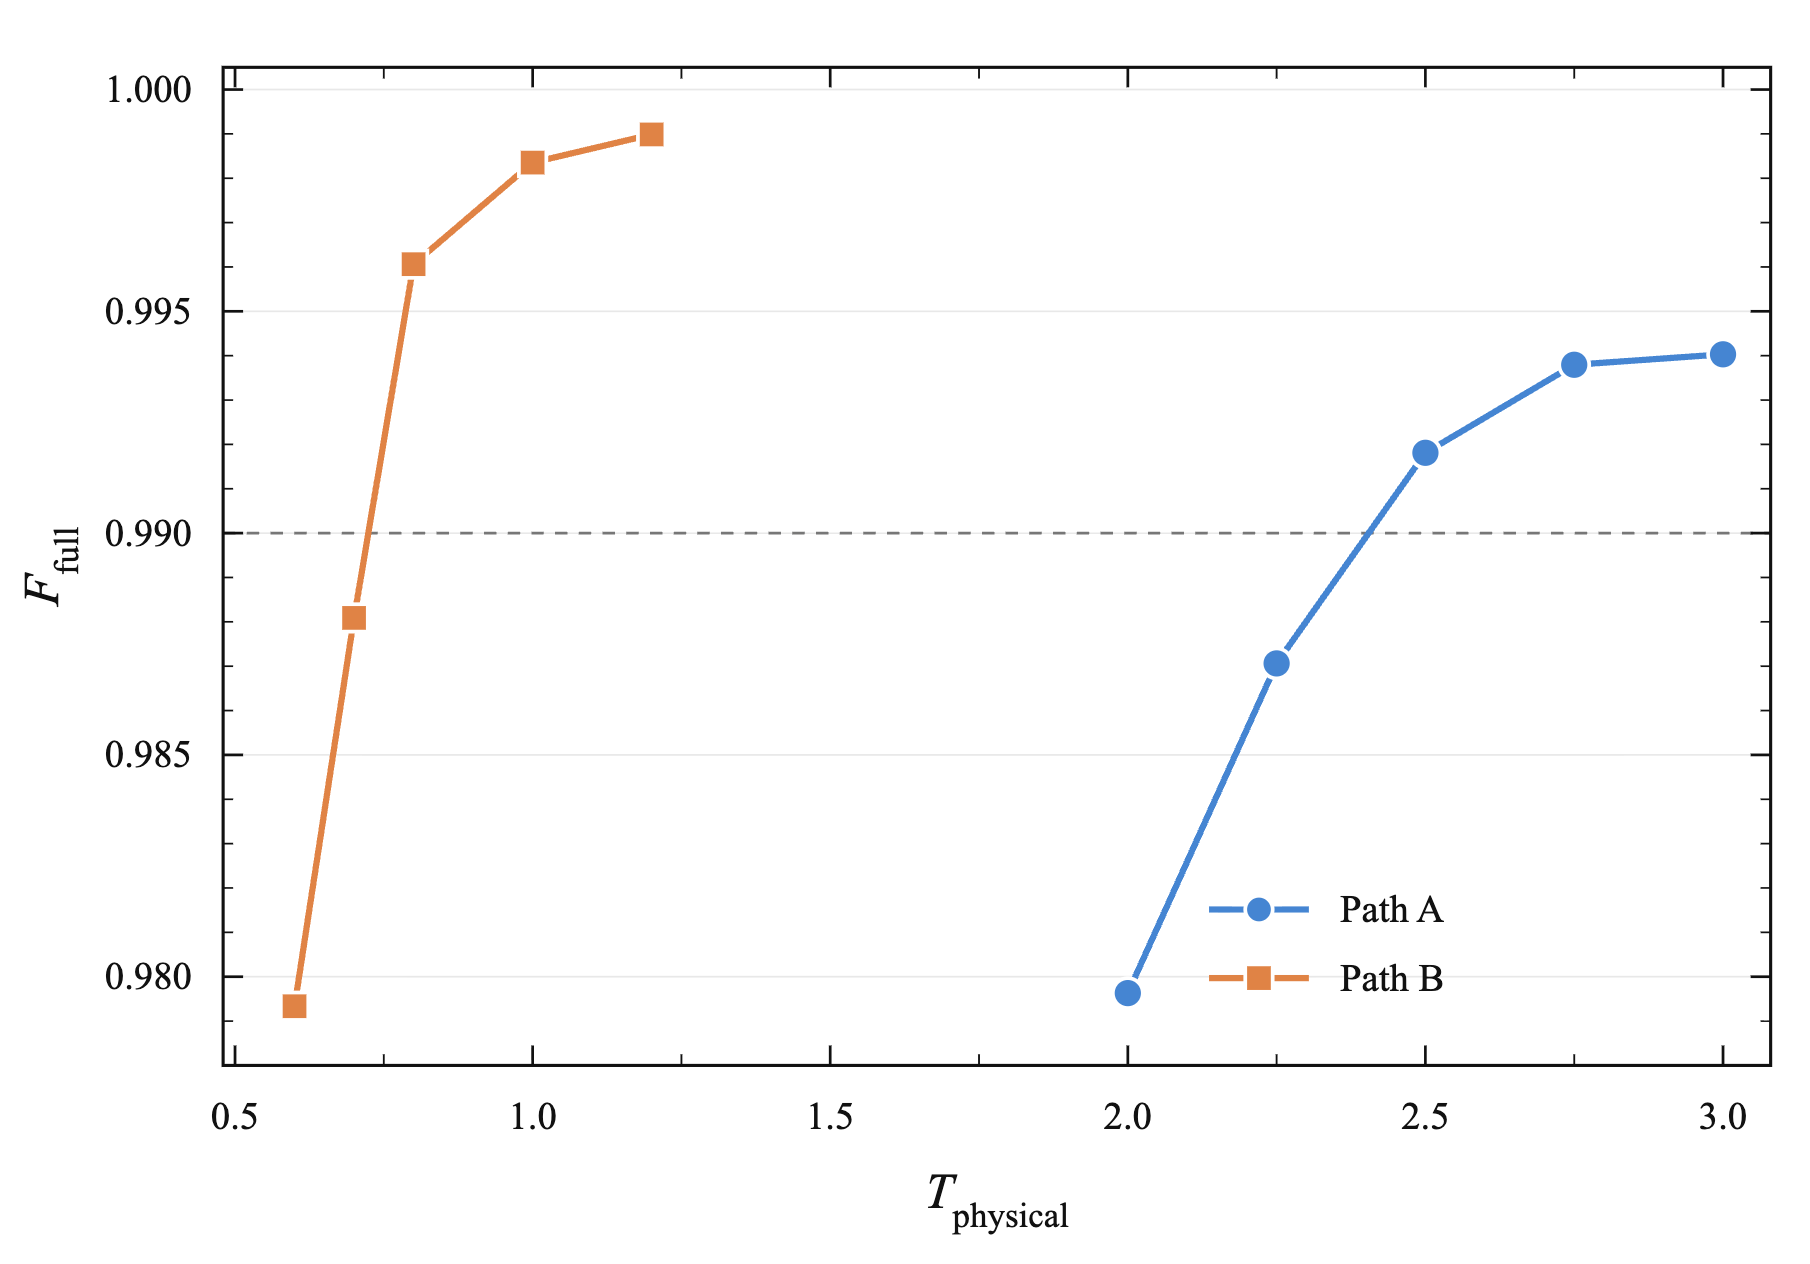
\includegraphics[width=0.6\columnwidth]{F_vs_t.png}
  \caption{The fidelity of the optimized curves verified using CF4-Krylov time evolution. Here $T_{\rm physical}= (T/75.69) \mu s$.}
  \label{fig:fidelity}
\end{figure}
We can calculate the relative error of the two-point function measured on the time-evolved states, as shown in~\ref{fig:rampingerror}.
\begin{figure}[t]
  \centering
  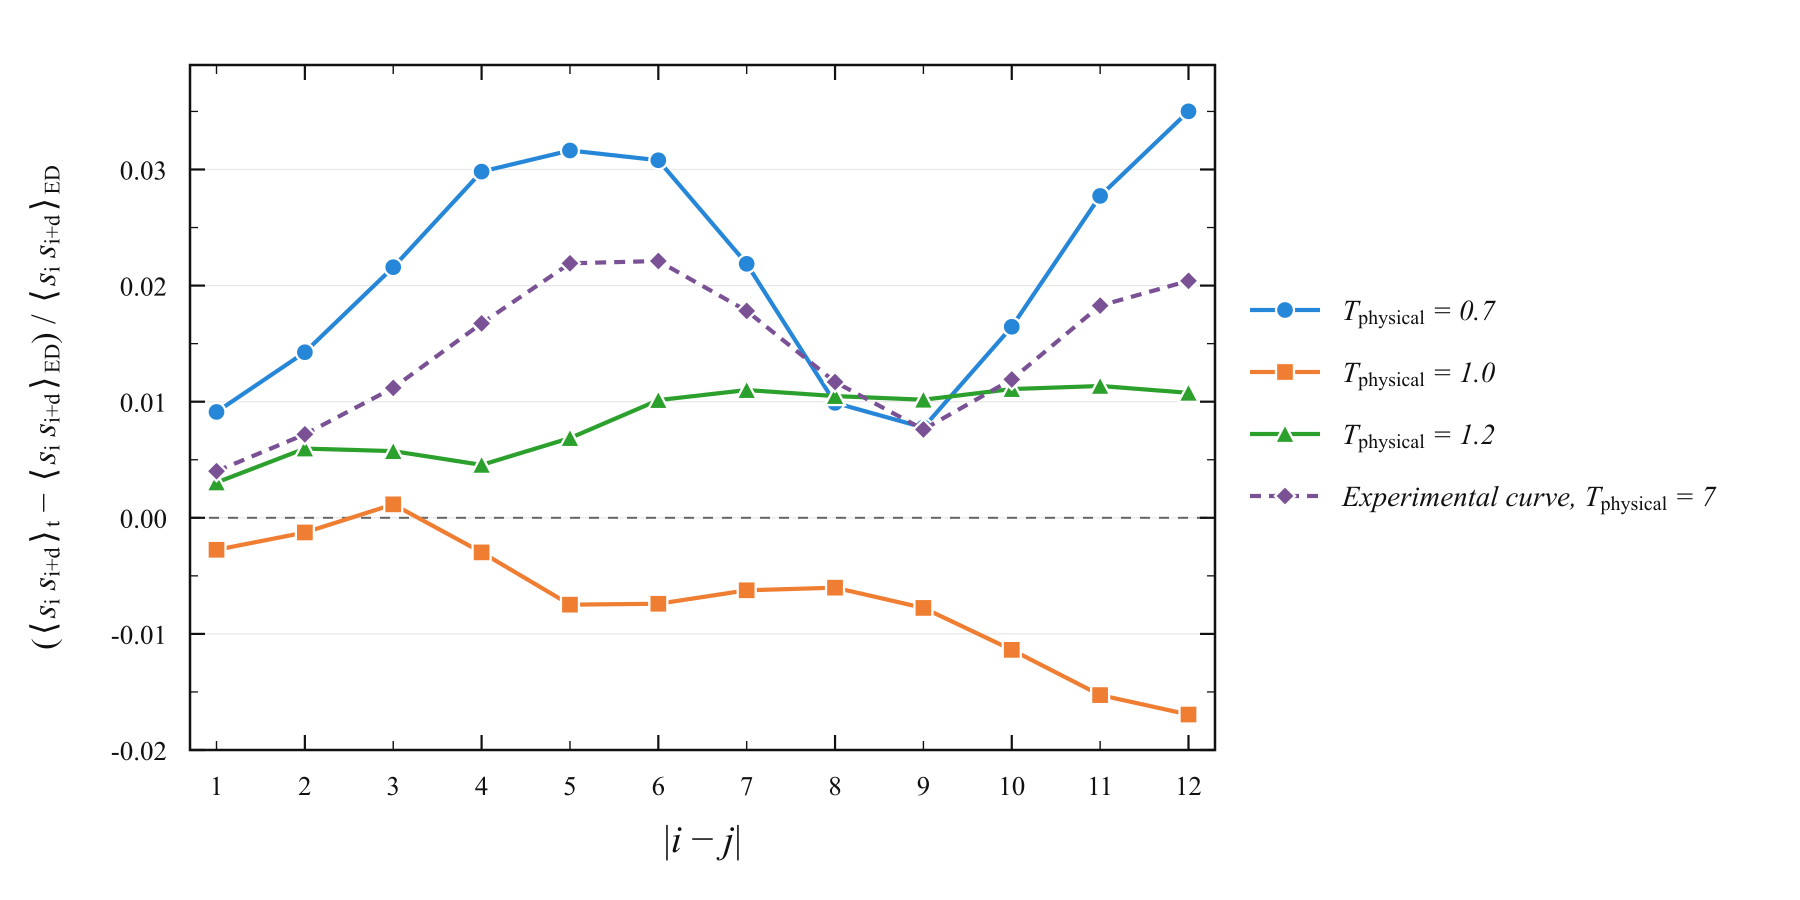
\includegraphics[width=0.9\columnwidth]{ramping_error.png}
  \caption{The relative error of the two-point function for the optimized curve of Path B and the experimental curve, as defined in~\eqref{def:error}. }
  \label{fig:rampingerror}
\end{figure}


\begin{table*}[t]
\centering
\caption{Optimized coefficients for Path A and Path B. The coefficients enter the
six-sine plus six-cosine time-density ansatz.}
\label{tab:path-coefficients}
\resizebox{\textwidth}{!}{%
\begin{tabular}{c*{12}{r}}
\toprule
$T_{\mathrm{physical}}$
& $a_1$ & $a_2$ & $a_3$ & $a_4$ & $a_5$ & $a_6$
& $b_1$ & $b_2$ & $b_3$ & $b_4$ & $b_5$ & $b_6$ \\
\midrule
2.00
&  0.565161 & -1.657209 &  3.299559 &  2.171572 & -1.762571 &  2.607463
& -3.832125 & -2.438523 & -5.717325 &  3.100494 & -1.826421 & -3.311279 \\
2.25
&  0.553266 & -0.634082 &  3.273120 &  4.607602 & -2.649089 &  0.498309
& -5.271103 & -2.026259 & -5.404912 &  3.881643 &  0.612730 & -3.308933 \\
2.50
& -0.096198 & -0.819855 &  2.688715 &  4.455646 & -2.987238 & -0.163164
& -5.604367 & -2.128336 & -4.931697 &  4.193614 &  1.601918 & -2.771219 \\
2.75
& -2.188016 & -0.907333 &  2.860120 &  4.814655 & -3.037231 & -0.667492
& -4.404842 & -2.495907 & -4.589297 &  4.883557 &  3.250500 & -1.941580 \\
3.00
& -0.699069 & -0.863736 &  2.237207 &  6.867565 & -1.721453 & -1.052913
& -6.161076 & -1.618110 & -4.648907 &  5.394653 &  5.997293 & -0.610818 \\
\bottomrule
\end{tabular}%
}
\resizebox{\textwidth}{!}{%
\begin{tabular}{c*{12}{r}}
\toprule
$T_{\mathrm{physical}}$
& $a_1$ & $a_2$ & $a_3$ & $a_4$ & $a_5$ & $a_6$
& $b_1$ & $b_2$ & $b_3$ & $b_4$ & $b_5$ & $b_6$ \\
\midrule
0.60
& -4.272404 & -0.257878 & -2.750781 &  0.761435 &  1.116412 &  0.187347
& -0.699790 &  0.540612 & -1.027274 & -2.483160 & -0.067789 &  0.669567 \\
0.70
& -4.594478 & -0.384034 & -3.139899 &  0.889628 &  1.209487 &  0.390048
& -0.976911 &  0.689999 & -0.813433 & -2.280804 &  0.058660 &  0.478638 \\
0.80
& -4.319620 & -0.460498 & -2.865799 &  0.875479 &  0.856311 &  0.419489
& -0.943799 &  0.679953 & -1.042947 & -2.369250 &  0.115863 &  0.407742 \\
1.00
& -4.248281 & -0.489297 & -3.012873 &  0.858625 &  0.689688 &  0.481482
& -1.004111 &  0.868316 & -0.946642 & -2.243263 &  0.298252 &  0.227596 \\
1.20
& -3.823077 & -0.660905 & -3.089450 &  0.664824 &  0.554296 &  0.733248
& -1.104026 &  1.132340 & -0.827626 & -2.207867 &  0.151625 &  0.041041 \\
\bottomrule
\end{tabular}%
}
\end{table*}

\bibliography{reference.bib}
\bibliographystyle{utphys}

\end{document}
